\documentclass[12pt]{article}
\setlength{\textwidth}{17cm}
\setlength{\textheight}{24cm}
\setlength{\topmargin}{-2cm}
\setlength{\footskip}{1cm}
\setlength{\evensidemargin}{0cm}
\setlength{\oddsidemargin}{0cm}
\setlength{\parindent}{0.75cm}

\usepackage{allrunes}
\usepackage{amsmath}
\usepackage[magyar]{babel}
\usepackage[T1]{fontenc}
\usepackage[utf8]{inputenc}
\usepackage{fixltx2e}
\usepackage{multirow}

\usepackage[hyphens]{url}
\usepackage[unicode,colorlinks=true,breaklinks]{hyperref}
%\usepackage[dvips]{hyperref}
%should display links, but it does not work with \H accent
%and formulas in section titles

\hypersetup{colorlinks,linkcolor=blue,urlcolor=magenta,citecolor=magenta}
%Breaks long url`s in text, while keeping it one link:

\usepackage{amsfonts}
\usepackage{amsthm}
\usepackage{amssymb}


\theoremstyle{plain}
\usepackage{graphicx}

%\usepackage{gensymb}
\usepackage{float}

% For bra-ket notation
\usepackage{braket}

%% New commands
\newcommand{\dd}{\textrm{d}}



\begin{document}
\title{15. tétel \\ Relációs adatbázisok}
\author{Bulatovic Nikola}

\maketitle

\begin{abstract}
     A relációs adatmodell, logikai és fizikai operátorok (seek, scan és a joinok változatai, aggregálás), adattárolási modellek (row store, column store), indexek (klaszterezett index, nem klaszterezett index), a B-fa, kulcsok és kényszerek, tranzakciók. Lekérdezésoptimalizálás. Az adatbetöltés menete. \par
     Ez a tétel az \textit{Adatmodellek és adatbázisok a tudományban} kurzus alapján készült \cite{db}. Megjegyzés: az utolsó fejezetek témakörei (Tranzakció kezelése c. fejezettől) nem szerepeltek az előadáson, így ezek nem szerepelnek részleteiben a tételben.
\end{abstract}

\tableofcontents
\newpage


\section{Bevezetés - adatbázis szerverek}

Az adatbázis szerver áltlában olyan dedikált szerver, amely különféle adatbázis szolgáltatásokat nyújt más gépeknek vagy programoknak a kliens-szerver modell alapján leírt módokon. Az ilyen szervereken a háttértár, az I/O és a hálózat konfigurációja erősen optimalizált. Az adatbázis szerver fő feladatai:
\begin{itemize}
    \item rendezett adattárolás a megmaradó (non-volatile) memóriában vagyis a háttértárolón
    \item lekérdezések (query) gyors végrehajtása
    \item adatmódosítás
    \item tranzakciók kezelése (hosszú, konkurens műveletek atomizált végrehajtása)
    \item adat konzisztencia fenntartása
    \item adatbiztonság (rendszerhiba esetén is megmaradó adatok)
\end{itemize}{}
Többféle adatbázis kezelő rendszer (database management system - DBMS) létezik, melyek ilyen adatbázis szerver funkcionalitással rendelkeznek. Az egyik legismertebb és legtöbbet használt a relációs adatbázis kezelő rendszerek (RDBMS). Ezeknek többféle implementációja létezik: Oracle, Microsoft SQL Server, vagy a nyílt forráskódú Postgres és MySQL. Ezek közös tulajdonsága, hogy mindegyik relációs adatmodellt alkalmaz, a lekérdezésekhez pedig egy adat-orientált deklaratív nyelvet az SQL-t (Structured Query Language) használ. 


\section{Relációs adatmodell}

Az adatbázisok logikai alapeleme a tábla (table). A táblák oszlopait a séma jellemzi: az adattípus és méret előre definiált. Az adatot magát a tábla sorai jelentik, amelyek száma tetszőleges és azonos formátumúak. A táblákon belül különböző megkötések lehetnek: 
\begin{itemize}
    \item[-]elsődleges kulcs (primary key), ami a táblán belül egyedi és egy vagy több oszlop kombinációja, mellyel a rendezés jól definiált (kulcsok összehasonlíthatóak <,>,=) 
    \item[-]másodlagos kulcs (foreign key), ami egy másik tábla elsődleges kulcsára mutat
\end{itemize}{}
Az adatbázisok működési logikáját a relációs adatmodell írja le, melynek matematikai alapja a relációs algebra. A relációs adatszerkezet alapfogalmai a következők:
\begin{itemize}
    \item \textbf{halmaz}: egy táblázat oszlopa, vagy oszlopok rendezett listája (tuple)
    \item \textbf{műveletek}: Descartes-szorzat, szelekció, projekció, unió, különbség
    \item \textbf{séma}: megkötés, hogy milyen halmazok, milyen sorrendben szorozhatóak össze
    \item \textbf{reláció}: Descartes-szorzat részhalmaza.
\end{itemize}{}
A logikai működést - matematikai precizitás mellőzve- úgy lehet összefoglalni, hogy a lekérdezések a táblázatok Descartes-szorzatán végzett műveletek utáni részhalmaz képzést jelent (\ref{fig:rel}. ábra).


\begin{figure}[H]
    \begin{center}
    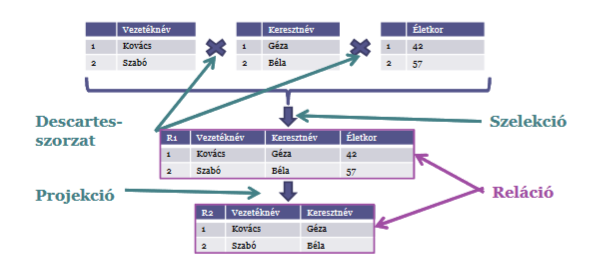
\includegraphics[width=0.85\textwidth]{media/rel.png}
    \caption{\textbf{A relációs algebra sematikus ábrázolása.} A lekérdezés végeredménye (reláció) a halmazok Descartes-szorzatának egy részhalmaza.} 
    \label{fig:rel}
    \end{center}
\end{figure}


\section{Adatok fizikai tárolása az adatbázis szerveren}

Az adatbázisok alapproblémai a következők:
\begin{itemize}
    \item[-] a háttértár mindig jóval lassabb, mint a központi memória és a CPU (megoldás: indexelés)
    \item[-] a háttértár szekvenciálisan sokkal gyorsabban olvasható, mint random módon
    (megoldás: sorok lapokba (page) szervezése,  lapok megfelelő sorrendben tárolása)
    \item[-] a memória mérete mindig sokkal kisebb, mint az adatbázis mérete (megoldás: ügyes algoritmusok, hogy ne kelljen transzformálni a memória és a diszken levő formátum között). 
\end{itemize}{}
Az adatok fizikai szervezésének megértése elengedhetetlen ahhoz, hogy lássuk hogyan kell a háttértárat és az adatbázist optimálisan konfigurálni. Sokszoros sebességnövekedés érhető el a naiv adatbázis szervezéshez képest. A  továbbiakban sor alapú adattárolás bemutatása következik. 
\\
\subsection{Lapok}
A fizikai egységek a következők: adatbázis > file group > file > extent > page, illetve a tranzakciós napló (lásd Tranzakciók fejezet). A tárolás alapegysége tehát a lap (\ref{fig:lap}. ábra):
\begin{itemize}
    \item[-] mérete fix 8kB
    \item[-] 8 lap alkot egy extent-et (64 kB)
    \item[-] csak teljes extent írható/olvasható a lemezre/ről
    \item[-] formátum a memóriában és a lemezen azonos
    \item[-] több fajtája van (tábla adat, index stb.)
\end{itemize}{}

\begin{figure}[H]
    \begin{center}
    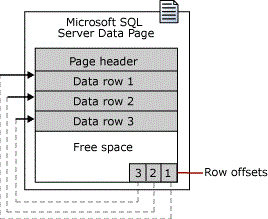
\includegraphics[width=0.55\textwidth]{media/page.png}
    \caption{\textbf{A tárolás alapegysége, a lap (page).} Az adatbázisban tárolt fájlok által allokált tárhely logikailag ilyen lapokra vannak osztva. Minden lap rendelkezik egy headerrel, amely tartalmazza a lap számát, típusát, a maradék üres hely méretét. A táblázat sorai a lapokon tárolódnak sorfolytonosan. Minden lap rendelkezik egy row offset táblázattal, ami megadja hogy a lapon szereplő sorok hányadik bájtnál kezdődnek a lap elejéhez képest.} 
    \label{fig:lap}
    \end{center}
\end{figure}

\subsection{Adatstruktúrák}
Ahogy korábban láttuk az adattárolás logikai egysége a tábla, azon belül pedig a sor. Ha egy tábla sorai nem meghatározott sorrendben tárolódnak (heap table), akkor egy új sor beírása könnyű (az utolsó lap végére kell írni), azonban kereséskor az egész táblát végig kell olvasni. Mint láttuk, az elsődleges kulcs használata egy lehetséges rendezést definiál a sorok között. Ha létezik egy ilyen rendezés, akkor táblát klaszterezett indexszel tárolhatjuk fizikailag.\par
Sorba rendezett adatok tárolására egy lehetséges adatstruktúra a B-fa, amely a hagyományos bináris-fa általánosítása. A bináris fa esetében egy új adatpont beírásakor gyakran az egész fát újra kell építeni, ami használhatatlanná teszi adatok diszken történő tárolására. A B-fa is csomópontokból áll, de az $d$ számú adatsort és $d+1$ számú pointert tartalmaz (bináris esetben $d = 1$). A pointerek további csomópontokra mutatnak, amelyekben található érték a pointer csomópontjában lévő adatok értékei közé esik (\ref{fig:tree}. ábra).

\begin{figure}[H]
    \begin{center}
    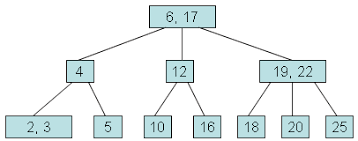
\includegraphics[width=0.65\textwidth]{media/btree.png}
    \caption{\textbf{A B-fa legegyszerűbb sematikus ábrázolása.}} 
    \label{fig:tree}
    \end{center}
\end{figure}

A B-fa építésekor ha egy csomópont betelik, akkor kettéosztjuk. Az ilyen módon konstruált fa egy ún. \textit{self balancing} kereső fa, ami azt jelenti hogy egy elem megtalálása (a fa mélysége) $\sim o(log_dn)$. A B-fa ezzel megoldja a bináris fa problémáit.
\par
Ennek ellenére néhány művelet a B-fa esetében is költséges lehet, a keresett csomópont mélységének függvényében. Ezt a problémát oldja fel a B-fa egy optimalizálás, a B+-fa. Ahelyett, hogy minden csomópontot egyformán kezelne, két típusba sorolja őket: a közbenső szinteken csak a kulcsokat és a pointereket tárolja, a tényleges adatokat csak a legalsó szinten. 
\\
Ezek alapján az adatbázis tábláit B+-fa struktúrában tárolhatjuk. A fa szintje egy lapnak felel meg. Mivel a B+-fa struktúrában kétféle csomópont van ehhez két fajta lapot igényel: index és sorokat tároló lap. A lapokon a pointerek a soron következő/előző lapokra mutat (\ref{fig:idx}. ábra). Ez a következő előnyökkel jár: 
\begin{itemize}
    \item[-] a tábla szekvenciálisan, a kulcs szerinti sorrendben (vagy visszafele) olvasható \\
    SELECT * FROM t WHERE id BETWEEN 12 AND 66
    \item[-] egy adott kulcsú sor gyorsan megtalálható \\SELECT * FROM t WHERE id = 12
    \item[-] egy adott kulcs tartomány gyorsan megtalálható, nem kell rendezni \\
    SELECT * FROM t ORDER BY id (ORDER BY elhagyható)
\end{itemize}{}

\section{Indexek}

\subsection{Nem klaszterezett indexek}
Ahogy az előzőekben láttuk egy táblához klaszterezett index építhető, amely jelentősen gyorsíthatja a lekérdezéseket. Egy táblán csak egy ilyen index lehet, amely meghatározza a tárolás sorrendjét. Az optimalizált lekérdezés csak az indexhez tartozó elsődleges kulcs alapján lehetséges, Ha más oszlop szerint is hasonló gyorsasággal szeretnénk keresni, akkor nem klaszterezett indexeket kell használunk.
\par
A nem klaszterezett index a tábla soraitól eltérő struktúrával rendelkezik, mivel az indexek sorrendje nem tükrözi az adatok fizikailag tárolt sorrendjét. Ehelyett az elsődleges kulcstól eltérő oszlop vagy oszlopokra épül és az ezek szerinti sorrendet indexeli. Ezek tárolási struktúrája hasonlóan B+-tree, azonban a fa utolsó (leaf) csomópontjai nem a tényleges adatot tárolják, hanem csak egy arra mutató pointert (\ref{fig:idx}. ábra).

\begin{figure}[H]
    \begin{center}
    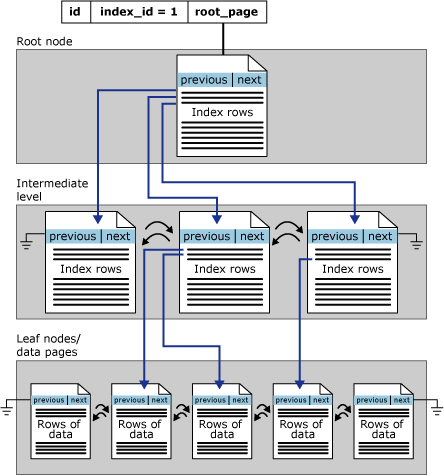
\includegraphics[width=0.45\textwidth]{media/cluster.png}
    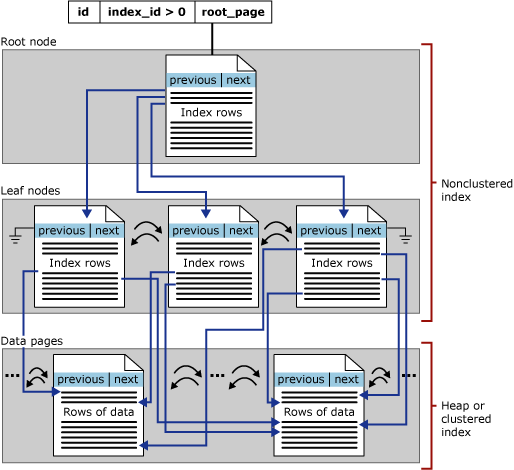
\includegraphics[width=0.5\textwidth]{media/noncluster.png}
    \caption{\textbf{Klaszterezett (bal) és nem klaszterezett index (jobb).} A klaszterezett index esetében a fa levelei a tényleges adatot tárolják. A nem klaszterezett index esetében pedig egy pointer található arra az adat page-re, amelyen a tényleges adat található. Ha a tábla nem rendelkezik klaszterezett indexszel, akkor a pointer heap page-re mutat, ahol az adat van.} 
    \label{fig:idx}
    \end{center}
\end{figure}

\subsection{Beágyazott oszlopok}

Ha olyan lekérdezést írunk, amihez csak az indexelt oszlopok kellenek, akkor elég csak az index struktúrát végigolvasni, az eredmény ezekből egyértelmű. Ha más oszlop is szerepel a lekérdezésben, akkor ezeket külön be kell tölteni a táblából.\par
Nem klaszterezett indexek létrehozásakor hozzáadhatunk beágyazott oszlopokat (included columns) az indexhez olyan formában, hogy az index pointerei mellé bekerülnek ezek az oszlopok is. Ekkor nem kell az adatsort külön betölteni kereséskor.

\subsection{Indexek tulajdonságai}

Indexek használatának előnyei:
\begin{itemize}
    \item[-]adott oszlopok szerinti keresés gyors, de csak ha a legelső indexelt oszlopra erős a megszorítás
    \item[-]az indexelt adatok az előírt sorrendben, szekvenciálisan olvashatóak.
\end{itemize}{}
Hátrányai:
\begin{itemize}
    \item[-]több tárhelyet igényel(az indexelt oszlopok még egyszer tárolódnak
    \item[-]beszúráskor, módosításkor, törléskor frissíteni kell
\end{itemize}{}








\section{Logikai és fizikai operátorok}
\section{Tranzakciók kezelése}
\section{Lekérdezésoptimalizálás}
\section{Az adatbetöltés menete}
\section{Oszlop alapú adattárolás}
130 old en


\bibliographystyle{plain}
\bibliography{references}

\end{document}
